\documentclass{article}

\usepackage{amsmath}
\usepackage{amssymb}
\usepackage{amsthm}
\usepackage{authblk}
\usepackage[english]{babel}
\usepackage{blkarray}
\usepackage[font=small]{caption}
\usepackage{cite}
\usepackage{graphicx}

% ---- Author affiliations ---- %

\renewcommand\Affilfont{\itshape\small}

% ---- Propositions, lemmas, defintions... ---- %

\newtheorem{algorithm}{Algorithm}
\newtheorem{corollary}{Corollary}
\newtheorem{definition}{Definition}
%\newtheorem{example}{Example}
\newtheorem{lemma}{Lemma}
\newtheorem{proposition}{Proposition}
%\newtheorem{remark}{Remark}


% ---- Special environments (examples and remarks) ---- %

\newcounter{examplecounter}
\newenvironment{example}
{\small\vspace{0.5\baselineskip}
  \refstepcounter{examplecounter}%
  \noindent\textbf{Example \arabic{examplecounter}.}%
}{\vspace{-0.2\baselineskip}\begin{center}%
  $\star$\end{center}\vspace{0.5\baselineskip}}

\newcounter{remarkcounter}
\newenvironment{remark}
{\small\it\vspace{0.5\baselineskip}
  \refstepcounter{remarkcounter}%
  \noindent\textbf{Remark \arabic{remarkcounter}.}%
}{\vspace{0.5\baselineskip}}

\newenvironment{inset}
{\vspace{0.5\baselineskip}\begin{center}}
{\end{center}\vspace{0.5\baselineskip}}


% ---- Macros ---- %

\newcommand{\DN}{\scriptstyle{\Downarrow}}
\newcommand{\dn}{\scriptstyle{\downarrow}}
\newcommand{\up}[1]{\scriptstyle{(\uparrow)_{#1}}}
\newcommand{\eq}[1]{\scriptstyle{(\sim)_{#1}}}

\newcommand{\upg}{\scriptstyle{\uparrow}}
\newcommand{\eqg}{\scriptstyle{\sim}}

%---------------------------------------------------------------

\title{Calibrating MEM seeding heuristics}

\author[1,2]{Guillaume J. Filion}
\affil[1]{Genome Architecture, Gene Regulation, Stem Cells and Cancer
Programme, Center for Genomic Regulation (CRG), The Barcelona Institute of
Science and Technology, Dr. Aiguader 88, Barcelona 08003, Spain.}
\affil[2]{University Pompeu Fabra, Doctor Aiguader, 08003 Barcelona,
Spain.}

\date{\today}

%---------------------------------------------------------------
%---------------------------------------------------------------


\begin{document}

\maketitle

\begin{abstract}
The abstract will come later.
\end{abstract}


%---------------------------------------------------------------
%---------------------------------------------------------------

\section{Introduction}
Some introduction

\section{MEM seeds}

\subsection{Seeds}
DEFINE MEM SEED AND SHARED MEM SEED.

EXPLAIN THAT THE TAIL IS AN UNTERMINATED SEGMENT.

\subsection{The seeding alphabet}

In order to compute seeding probabilities, we need to consider that reads
are sequences of letters from the \emph{seeding alphabet} rather than from
the nucleotide alphabet. them as a sequence of symbols telling if the
nucleotides match the target and~/ or the duplicates. Here, we will
consider that reads are sequences of the five symbols $\Downarrow$,
$\downarrow$, $\uparrow$, $\sim$ and $\square$.

The $\Downarrow$ symbol indicates that the nucleotide is not only a
mismatch for the target, but also for every duplicate. The $\downarrow$
symbol indicates that the nucleotide is a mismatch for the target, but is
a match for at least one dupulicate. These two symbols are referred to as
the \emph{error symbols}, because they imply the occurrence of a
sequencing error (this is the only way the read may not match the target).

The remaing three symbols have a more complex usage because they describe
events of the MEM seeding process that are best explained by way of a
concrete example. Fig.~\ref{fig:sketch_MEM} illustrates the case of a read
of size 25 from a sequence with three duplicates. The four files of
squares at the bottom are the target and duplicate sequences, where a
black square means that the decoded nucleotide is a mismatch and a grey
square means that it is a match.


\begin{figure}[h]
\centering
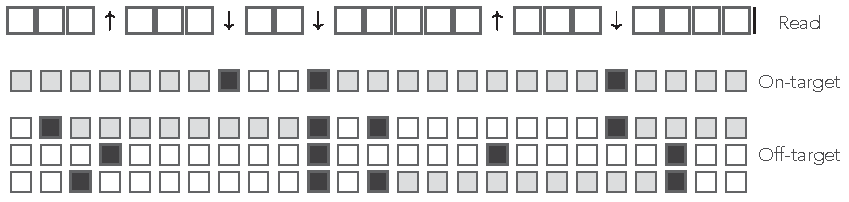
\includegraphics[scale=.9]{sketch_MEM.pdf}
\caption{\textbf{Reads and MEM seeds}. 
Some legend.}
\label{fig:sketch_MEM}
\end{figure}

Now consider streaks of matches until a particular position of the read.
At the 4-th nucleotide, the target scores 4 matches in a row versus 2, 0
and 1 for the duplicates. The target just acquired the strictly longest
streak, which is indicated by the $\uparrow$ symbol. This symbol also
appears at position 17, where the target sequence acquires the strictly
longest streak again (6 matches in a row, versus 4, 0 and 4 for the
dupicates).

At position 23, the target and the first duplicate both acquire the
longest streak (2 matches in a row), which is indicated by the $\sim$
symbol. This symbol is used only at positions where the target
\emph{acquires} the longest streak (together with at least one duplicate).
For instance, it is not used at position 1 nor at position 12 because the
target already had the longest streak (0 in both cases).

Finally, the $\square$ symbol is used for all the other cases,
\textit{i.e.}, when there is no sequencing error, and when the target does
not acquire the longest streak of matches (shared or not with a
duplicate).

Each sequence corresponds to a Bernoulli process where `success' stands
for a match between the sequence and the read, and `failure' stands for a
mismatch. For simplicity, we will refer to the Bernoulli processes as
`threads'.

\begin{definition}
At a given position of the read, a duplicate thread is said to be
\emph{strictly masking} if its success streak is strictly longer than the
match streak of the target. A duplicate thread is said to be
\emph{potentially masking} if its match streak is the same as the target.
\end{definition}

Duplicate threads are thus classified into strictly masking, potentially
masking and not masking, which allows us to describe the usage of the five
symbols.

\begin{figure}[h]
\centering
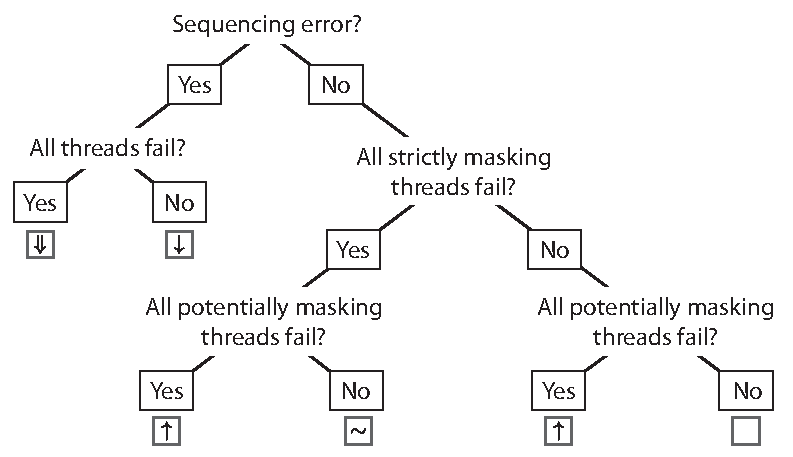
\includegraphics[scale=.7]{decision_tree.pdf}
\caption{\textbf{Decision tree}. 
Some legend.}
\label{fig:decision_tree}
\end{figure}


We assume that the target sequence has $N$ duplicates that are potential
false positives for the seeding process. We further assume that
duplication was instantaenous and that all $N+1$ sequences diverge
independently from each other at a constant rate. In other words, we
ignore the complications due to the genealogy of the duplication events
and we simply assume that at each position, any given duplicate has the
same nucleotide as the target with probability $1-\mu$. If it does not,
we assume that the duplicate has any of the remaining three
nucleotides with equal probability.

To describe those processes, we will
often use the function $\varphi(n)$ that gives the length of the success
streak at position $n$. The processes are indexed such that $\varphi_0$
refers to the target sequence, and functions $\varphi_j$ $(1 \leq j \leq
N)$ refer to the duplicates. For a concrete example, $\varphi_0(5) = 5$
and $\varphi_1(5) = 3$ in Fig.~\ref{fig:sketch_MEM}.



With these definitions, the decision tree for choosing the next symbol to
insert in a read can be summarized as in Fig.~\ref{fig:decision_tree}.
This sketch will be useful as a reference to compute the probabilities of
the blocks and their weighted generating functions.




\begin{definition}
The main thread is dominant at nucleotide $n$ if $\varphi_0(n) >
\varphi_i(n)$ for all $i$ $(1 \leq i \leq N)$. The main thread is
co-dominant if inequality is not strict and there exists $i$ $(1\leq i
\leq N)$ such that $\varphi_0(n) = \varphi_i(n)$.
\end{definition}



%\begin{figure}[h]
%\centering
%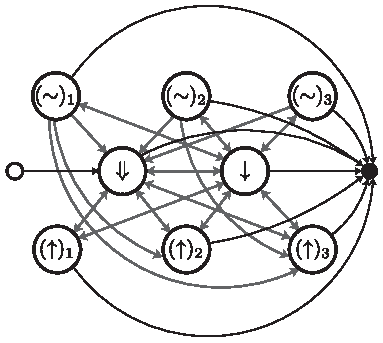
\includegraphics[scale=1]{no_3MEM_graph.pdf}
%\caption{\textbf{Transfer graph of a read without 3-MEM}. 
%Some legend.}
%\label{fig:noMEM_graph}
%\end{figure}



\section{The transfer matrix}

\subsection{Transitions from $\uparrow$}
\label{sec:trans_from_up}

On a $\uparrow$ symbol, the main thread becomes dominant. It will remain
so until the first sequencing error, so the next block will be terminated
by an error symbol (\textit{i.e.} $\Downarrow$ or $\downarrow$).

\begin{definition}
$\omega$ and $\tilde{\omega}$ are the probabilities of the $\Downarrow$
and of the $\downarrow$ error symbols, respectively, \textit{i.e.}
\begin{eqnarray}
\omega &=& p \cdot (1-\mu/3)^N \\
\tilde{\omega} &=& p \cdot \big( 1-(1-\mu/3)^N \big).
\end{eqnarray}
\end{definition}

The weighted generating function of the transition from $(\uparrow)_j$ to
$\Downarrow$ is
\begin{equation}
C^\Downarrow_j(z) = \omega z \sum_{i=0}^{\gamma-j-1} (qz)^i.
\end{equation}

The weighted generating function of the transition from
$(\uparrow)_j$ to $\downarrow$ is
\begin{equation}
C^\downarrow_j(z) = \tilde{\omega} z
  \sum_{i=0}^{\gamma-j-1} (qz)^i.
\end{equation}


\subsection{Transitions from $\Downarrow$}
\label{sec:trans_from_Down}

At a $\Downarrow$ symbol, all the threads have match length $0$ and the
read is `reset' to its initial state. The main thread is co-dominant with
all the alternative threads. The next terminator symbol depends on what
happens first. If all the alternative threads fail before the main thread,
the latter becomes dominant ($\uparrow$ symbol). If not all alternative
threads have failed when the main thread does, we need to distinguish two
cases: if all threads fail together with the main thread, the read is
reset ($\Downarrow$ symbol), otherwise the main read becomes dominated
($\downarrow$ symbol).

If the next terminator is the $\uparrow$ symbol, we need to distinguish
the cases based on the value of $\varphi_0$ (see
section~\ref{sec:trans_from_up}), which is just the position of the
$\uparrow$ symbol after the $\Downarrow$ symbol in this case. A transition
from $\Downarrow$ to $(\uparrow)_j$ consists of a succession of $j$
correct nucleotides -- each with probability $q$. But we must also make
sure that no other $\uparrow$ symbol is inserted before position $j$.

\begin{definition}
$\xi_{i,m}$ is the probability that at least one of $m$ alternative
threads does not fail in $i$ error-free nucleotides, \textit{i.e.}
\begin{equation}
  \xi_{i,m} = 1-(1-(1-\mu)^i)^m.
\end{equation}
\end{definition}

The weighted generating function of the transition from $\Downarrow$ to
$(\uparrow)_i$ is
\begin{equation}
\label{eq:u}
u_i(z) = (\xi_{i-1,N}-\xi_{i,N})(qz)^i.
\end{equation}

\begin{remark}
If $N = 0$, the states $(\downarrow)_2, \ldots, (\downarrow)_{\gamma-1}$
are inacessible. Consistently, the mononomial $u_i(z)$ is equal to $qz$ if
$i = 1$ and $0$ otherwise.
\end{remark}

If the next terminator is $\Downarrow$, there is a limit on the
number of $\square$ symbols. Indeed, if there are $\gamma$ or more
nucleotides between the two $\Downarrow$ symbols, they constitute a shared
MEM seed. As mentioned in section~\ref{sec:trans_from_up}, the weighted
generating function of the $\Downarrow$ symbol is $pz(1-\mu/3)^N$. By the
same rationale as above, the weighted generating function of the
transition from $\Downarrow$ to $\Downarrow$ is
\begin{equation}
A^\Downarrow(z) = \omega z
  \sum_{i=0}^{\gamma-1} \xi_{i,N} \cdot (qz)^i.
\end{equation}


If the next terminator is $\downarrow$ we have to dinstinguish two cases.
In the example below, there is a shared MEM seed only if $\gamma \leq
11$. The main thread is unmasked, so the number of nucleotides between the
error symbols matters.
\begin{inset}
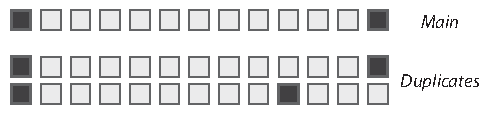
\includegraphics[scale=.9]{ddown_to_down_case_1.pdf}
\end{inset}
In this other example, there can be no MEM seed because the first
duplicate masks the main thread. This depends neither on the value of
$\gamma$ nor on the number of nucleotides between the error symbols.
\begin{inset}
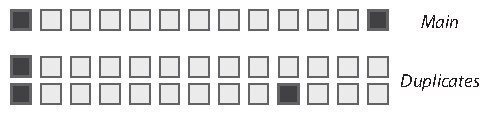
\includegraphics[scale=.9]{ddown_to_down_case_2.pdf}
\end{inset}

So if the $\Downarrow$ and the $\downarrow$ symbols are separated by
$\gamma-1$ or fewer nucleotides, there is no MEM seed and we must only
rule out the presence of other terminators in the segment (in this case
the $\uparrow$ symbol). The weighted generating function is
\begin{equation}
\tilde{\omega} z \sum_{i=0}^{\gamma-1} \xi_{i,N} \cdot (qz)^i.
\end{equation}

On the other hand, if the $\Downarrow$ and the $\downarrow$ symbols are
separated by $\gamma$ or more nucleotides, there could be a shared MEM
seed, so we must enforce the condition that at least one potentially
masking thread masks the main thread up to and including the $\downarrow$
symbol (this incidentally rules out the presence of other terminators in
the segment).

\begin{definition}
$\alpha_i$ is the probability that the first thread has at least one
failure in $i$ error-free nucleotides, followed by a sequencing error,
\textit{i.e.}
\begin{equation}
\alpha_i = 1 - (1-\mu)^i\mu/3
\end{equation}
\end{definition}

The probability that at least one duplicate thread masks the main thread
if the first error occurs at position $i$ is thus $1 - \alpha_{i-1}^N$.
The weighted generatin function is
\begin{equation}
pz\sum_{i=\gamma}^\infty (1 - \alpha_i^N) \cdot (qz)^i.
\end{equation}

Finally, the weighted generating function of the transition from
$\Downarrow$ to $\downarrow$ is
\begin{equation}
A^\downarrow(z) =
\tilde{\omega} z \sum_{i=0}^{\gamma-1} \xi_{i,N} \cdot (qz)^i +
pz\sum_{i=\gamma}^\infty (1 - \alpha_i^N) \cdot (qz)^i.
\end{equation}

\subsection{Transitions from $\downarrow$}
\label{sec:trans_from_down}

At a $\downarrow$ symbol, the main thread fails and at least one duplicate
thread does not (othwerwise the symbol would be $\Downarrow$). By
definition, the duplicate threads that do not fail are strictly masking,
and those that fail are potentially masking. A $\downarrow$ symbol implies
the presence of a sequencing error, so duplicate threads fail with
probability $1-\mu/3$. The probability that $m$ duplicate threads fail and
$N-m$ do not $(0 \leq m \leq N-1)$ is thus
\begin{equation}
  Q_m = \frac{1}{1-(1-\mu/3)^N}{N \choose m} (1-\mu/3)^m(\mu/3)^{N-m}.
\end{equation}

The probability that the next terminator is the $\uparrow$ symbol at
position $i$ is the probability that the last of the $N$ duplicate threads
fails at position $i$ is $\xi_{i-1,N-m}-\xi_{i,N-m}$ so the weighted
generating function of the transition from $\downarrow$ to $(\uparrow)_i$
is
\begin{equation}
\tag{\ref{eq:u}}
u_i(z) = (\xi_{i-1,N}-\xi_{i,N}) \cdot (qz)^i.
\end{equation}

To compute the weighted generating function of the transition from
$\downarrow$ to $\Downarrow$, we need to separate two cases. In the first,
the error symbols are separated by $\gamma-1$ or fewer error-free
nucleotides. In this case, there can be no MEM seed and we only have to
exclude the $\uparrow$ terminator. We obtain
\begin{equation}
\omega z \sum_{i=0}^{\gamma-1}\xi_{i,N} \cdot (qz)^i.
\end{equation}

In the case that $\downarrow$ and $\Downarrow$ are separated by $\gamma$
or more error-free nucleotides, we must ensure that at least one strictly
masking thread survives until the penultimate nucleotide of the segment.
This probability is equal to
\begin{equation}
\sum_{m=0}^{N-1}Q_m \cdot \xi_{i,N-m} =
\frac{1-\alpha_i^N}{1-(1-\mu/3)^N}.
\end{equation}

\begin{remark}
A strictly masking thread survives until the $\Downarrow$ symbol if and
only if one of the $N$ duplicate threads reverse-survives from
the penultimate nucleotide of the segment down to and including the
$\downarrow$ symbol.
\end{remark}

In sum, the weighted generating function of the transition from
$\downarrow$ to $\Downarrow$ is
\begin{equation}
B^\Downarrow(z) = 
\omega z \sum_{i=0}^{\gamma-1}\xi_{i,N} \cdot (qz)^i +
\omega z\sum_{i=\gamma}^\infty \frac{1-\alpha_i^N}{1-(1-\mu/3)^N} (qz)^i.
\end{equation}

If the next terminator is $\downarrow$, we again have to distinguish two
cases. If the two $\downarrow$ symbols are separated by $\gamma-1$ or
fewer nucleotides, there is no MEM seed and we must only rule out the
presence of the $\uparrow$ terminator. We obtain
\begin{equation}
\tilde{\omega} z\sum_{i=0}^{\gamma-1}
\xi_{i,N} \cdot (qz)^i.
\end{equation}

If the two $\downarrow$ symbols are separated by $\gamma$ or more
nucleotides, there could be a shared MEM seed, so we must enforce the
condition that the main thread is masked. This is satisfied if and only if
one of the following conditions holds:
\begin{enumerate}
\item A strictly masking thread survives until the penultimate
nucleotide of the segment.
\item All the strictly masking threads fail before the penultimate
nucleotide but a potentially masking thread survives until the last
nucleotide of the segment.
\end{enumerate}

Assuming that there are $m \geq 0$ potentially masking threads, the
probability of condition $1.$ is $\xi_{i-1,N-m}$ and that of condition 2.
is $(1-\xi_{i-1,N-m}) (1-\alpha_{i-1}^m)$. Summing of $m = 0, \ldots, N-1$
on obtains
\begin{equation}
(1-\mu/3)\sum_{m=0}^{N-1}Q_m \cdot \xi_{i-1,N-m} =
1-\alpha_{i-1}^N \text{, and}
\end{equation}
\begin{equation}
\sum_{m=0}^{N-1}Q_m (1-\xi_{i-1,N-m}) (1-\alpha_{i-1}^m) =
\frac{\alpha_{i-1}^N - \alpha_0^N -
  \zeta_{i-1,i-1}^N + \zeta_{0,i-1}^N}{1-(1-\mu/3)^N},
\end{equation}
where
\begin{equation}
\zeta_{j,i} = 1-(1-\mu)^j\mu/3-(1-\mu)^i\mu/3(1-\mu/3)
\end{equation}

Finally, the weighted generating function of the transitions from
$\downarrow$ to $\downarrow$ is
\begin{equation*}
B^\downarrow(z) = \tilde{\omega}z \sum_{i=0}^{\gamma-1} \xi_{i,N} \cdot
(qz)^i + pz \sum_{i=\gamma}^\infty
\left( 1-\alpha_i^N +
\frac{\alpha_i^N - \alpha_0^N - \zeta_{i,i}^N +
\zeta_{0,i}^N}{1-(1-\mu/3)^N} \right) (qz)^i
\end{equation*}

\begin{remark}
One can interpret $\zeta_{i,i}$ as the probability that
\end{remark}


\subsection{Head and tail vectors}

At the beginning of the read, the match lengths of all the threads are
$0$. This is exactly the same as on a $\Downarrow$ symbol. We can thus
consider that the read starts in the $\Downarrow$ state, which is
equivalent to adding an edge labelled with the empty object $\varepsilon$
between the head vertex and the $\Downarrow$ vertex. The head vector is
thus
\begin{equation*}
H(z) = 
\begin{blockarray}{ccccc}
   \;\; \DN & \dn & \up{1} & \ldots & \up{\gamma-1} \\
\begin{block}{[ccccc]}
\;\; 1 & 0 & 0 & \ldots & 0 \\
\end{block}
\end{blockarray}.
\end{equation*}
The tail vector contains the weighted generating functions of
non-terminated stretches of $\square$ symbols. Referring to the decision
tree of Fig.~\ref{fig:decision_tree}, we see that the probability of
occurrence of $\square$ symbols depends on whether there are potentially
masking and / or strictly masking threads. All the symbols except
$\downarrow$ impose a maximum on the number of $\square$ symbols at the
end of the reads.

For the $\downarrow$ symbol, the weighted generating function is
\begin{equation}
T^\downarrow(z) = 
\sum_{i=0}^{\gamma-1}\xi_{i,N} \cdot (qz)^i +
\sum_{i=\gamma}^\infty \frac{1-\alpha_i^N}{1-(1-\mu/3)^N} (qz)^i.
\end{equation}

For the $(\uparrow)_j$ state, the weighted generating function is
\begin{equation}
T^\uparrow_j(z) = \sum_{i=0}^{\gamma-j-1} (qz)^i.
\end{equation}

For the other symbols, we must take care that the potentially masking
threads do not all fail (otherwise this would imply the presence of a
$\uparrow$ terminator in the tail). For the $\Downarrow$ symbol, the
weighted generating function is
\begin{equation}
T^\Downarrow(z) = \sum_{i=0}^{\gamma-1} \xi_{i,N} \cdot (qz)^i.
\end{equation}

In summary,
\begin{equation*}
T(z) = 
\begin{blockarray}{cc}
\begin{block}{c[c]}
\DN & T^\Downarrow(z) \\
\dn & T^\downarrow(z) \\
\up{\gamma-1} & T^\uparrow_{\gamma-1}(z) \\
\vdots & \vdots \\
\up{1} & \; T^\uparrow_1(z) \; \\
\end{block}
\end{blockarray}.
\end{equation*}


\section{Conclusion}

\begin{equation*}
\begin{blockarray}{cccccc}
   & \DN & \dn & \up{1} & \ldots & \up{\gamma-1} \\
\begin{block}{c[ccccc]}
\DN & A^\Downarrow(z) & A^\downarrow(z) & u_1(z)
    & \ldots & u_{\gamma-1}(z) \\
\dn & B^\Downarrow(z) & B^\downarrow(z) & u_1(z)
    & \ldots & u_{\gamma-1}(z) \\
\up{1} & C_{\gamma-1}(z) & \tilde{C}_{\gamma-1}(z) & 0 &
    \ldots & 0 \\
\vdots & \vdots & \vdots & \vdots & \ddots & \vdots \\
\up{\gamma-1} & C_1(z) & \tilde{C}_1(z) & 0 & \ldots & 0 \\
\end{block}
\end{blockarray}
\end{equation*}

In the case $N = 0$, the symbol $\downarrow$ also disappears. Some
polynomials have a particularly simple form in this case, and the
body of the transfer matrix is
\begin{equation*}
\begin{blockarray}{ccc}
   & \DN & \up{1} \\
\begin{block}{c[cc]}
\DN    & pz              & qz \\
\up{1} & C_{\gamma-1}(z) & 0  \\
\end{block}
\end{blockarray}
\end{equation*}


\section*{Acknowledgements}

I acknowledge the financial support of the Spanish Ministry of Economy and
Competitiveness (‘Centro de Excelencia Severo Ochoa 2013-2017’, Plan
Nacional BFU2012-37168), of the CERCA Programme~/~Generalitat de
Catalunya, and of the European Research Council (Synergy Grant 609989).


%---------------------------------------------------------------
%---------------------------------------------------------------

\bibliography{references,pubmed}
\bibliographystyle{plain}

%----------------------------------------------------------------

\end{document}

%gs -dNoOutputFonts -sDEVICE=pdfwrite -o out.pdf latex.pdf 
